\documentclass[a4paper,12pt]{article}
\usepackage[T1]{fontenc}
\usepackage[polish]{babel}
\usepackage{amsmath, amssymb}
\usepackage{physics}
\usepackage{graphicx}
\usepackage{float}
\usepackage{geometry}
\geometry{left=25mm, right=25mm, top=25mm, bottom=25mm}
\graphicspath{{images/}{./}}

\begin{document}

\title{Podstawy mechaniki kwantowej}
\author{Notatki z wykładu}
\date{\today}
\maketitle
\tableofcontents

\section{Historia powstania fizyki kwantowej}

\subsection{Zapomnijmy o mechanice klasycznej}
Związek z nią będzie jasny, kiedy pójdziemy głębiej w teorię.

\subsection{Promieniowanie ciała doskonale czarnego}
Eksperyment Stefana-Boltzmanna (1878) badał promieniowanie cieplne emitowane przez ciało doskonale czarne.
Ciało doskonale czarne to obiekt, który pochłania całe promieniowanie i emituje je zgodnie z temperaturą.
\begin{figure}[H]
    \centering
    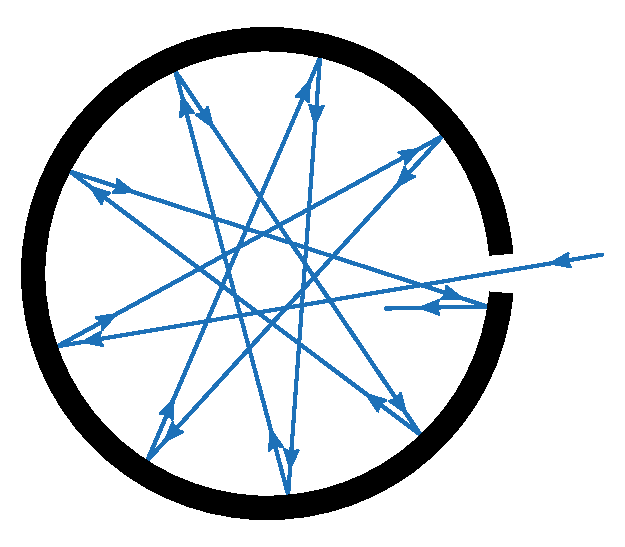
\includegraphics[width=0.3\textwidth]{blackbody}
    \caption{Ciało doskonale czarne. \textit{Źródło: Wikipedia}}
    \label{fig:blackbody}
\end{figure}

Pokazano, że całkowita energia wypromieniowywana przez takie ciało jest proporcjonalna do czwartej potęgi jego temperatury absolutnej
\begin{equation*}
    R(T) = \sigma T^4,
\end{equation*}
gdzie $R$ to moc promieniowania na jednostkę powierzchni, $T$ to temperatura w kelwinach, a $\sigma$ to stała Stefana-Boltzmanna.

Całkowita moc promieniowania to
\begin{equation*}
    R(T) = \int_0^\infty \rho(\lambda, T) d\lambda,
\end{equation*}
gdzie $\lambda$ to długość fali, a $\rho(\lambda, T)$ to spektralna funkcja rozkładu.

W 1893 Wien zauważył, że spektralna gęstość promieniowania nie zależy od $\lambda$ i $T$ osobno, ale od ich iloczynu $\lambda T$
\begin{equation*}
    \rho(\lambda, T) = \lambda^{-5} f(\lambda T).
\end{equation*}

\subsection{Prawo Rayleigha-Jeansa}
W klasycznej elektrodynamice, promieniowanie elektromagnetyczne opisane jako fale stojące daje rozkład energii w funkcji długości fali.
Liczba takich fal o długości od $\lambda$ do $\lambda + d\lambda$ to
\begin{equation*}
    \rho(\lambda, T) = \frac{8\pi}{\lambda^4} \cdot \bar{\epsilon},
\end{equation*}
gdzie $\bar{\epsilon}$ to średnia energia takiej fali.
Wzór ten jest dokładny dla długich fal, ale prowadzi do problemu z ,,katastrofą ultrafioletową'' przy krótkich falach, co zostało skorygowane przez teorię kwantową Plancka.

\begin{figure}[H]
    \centering
    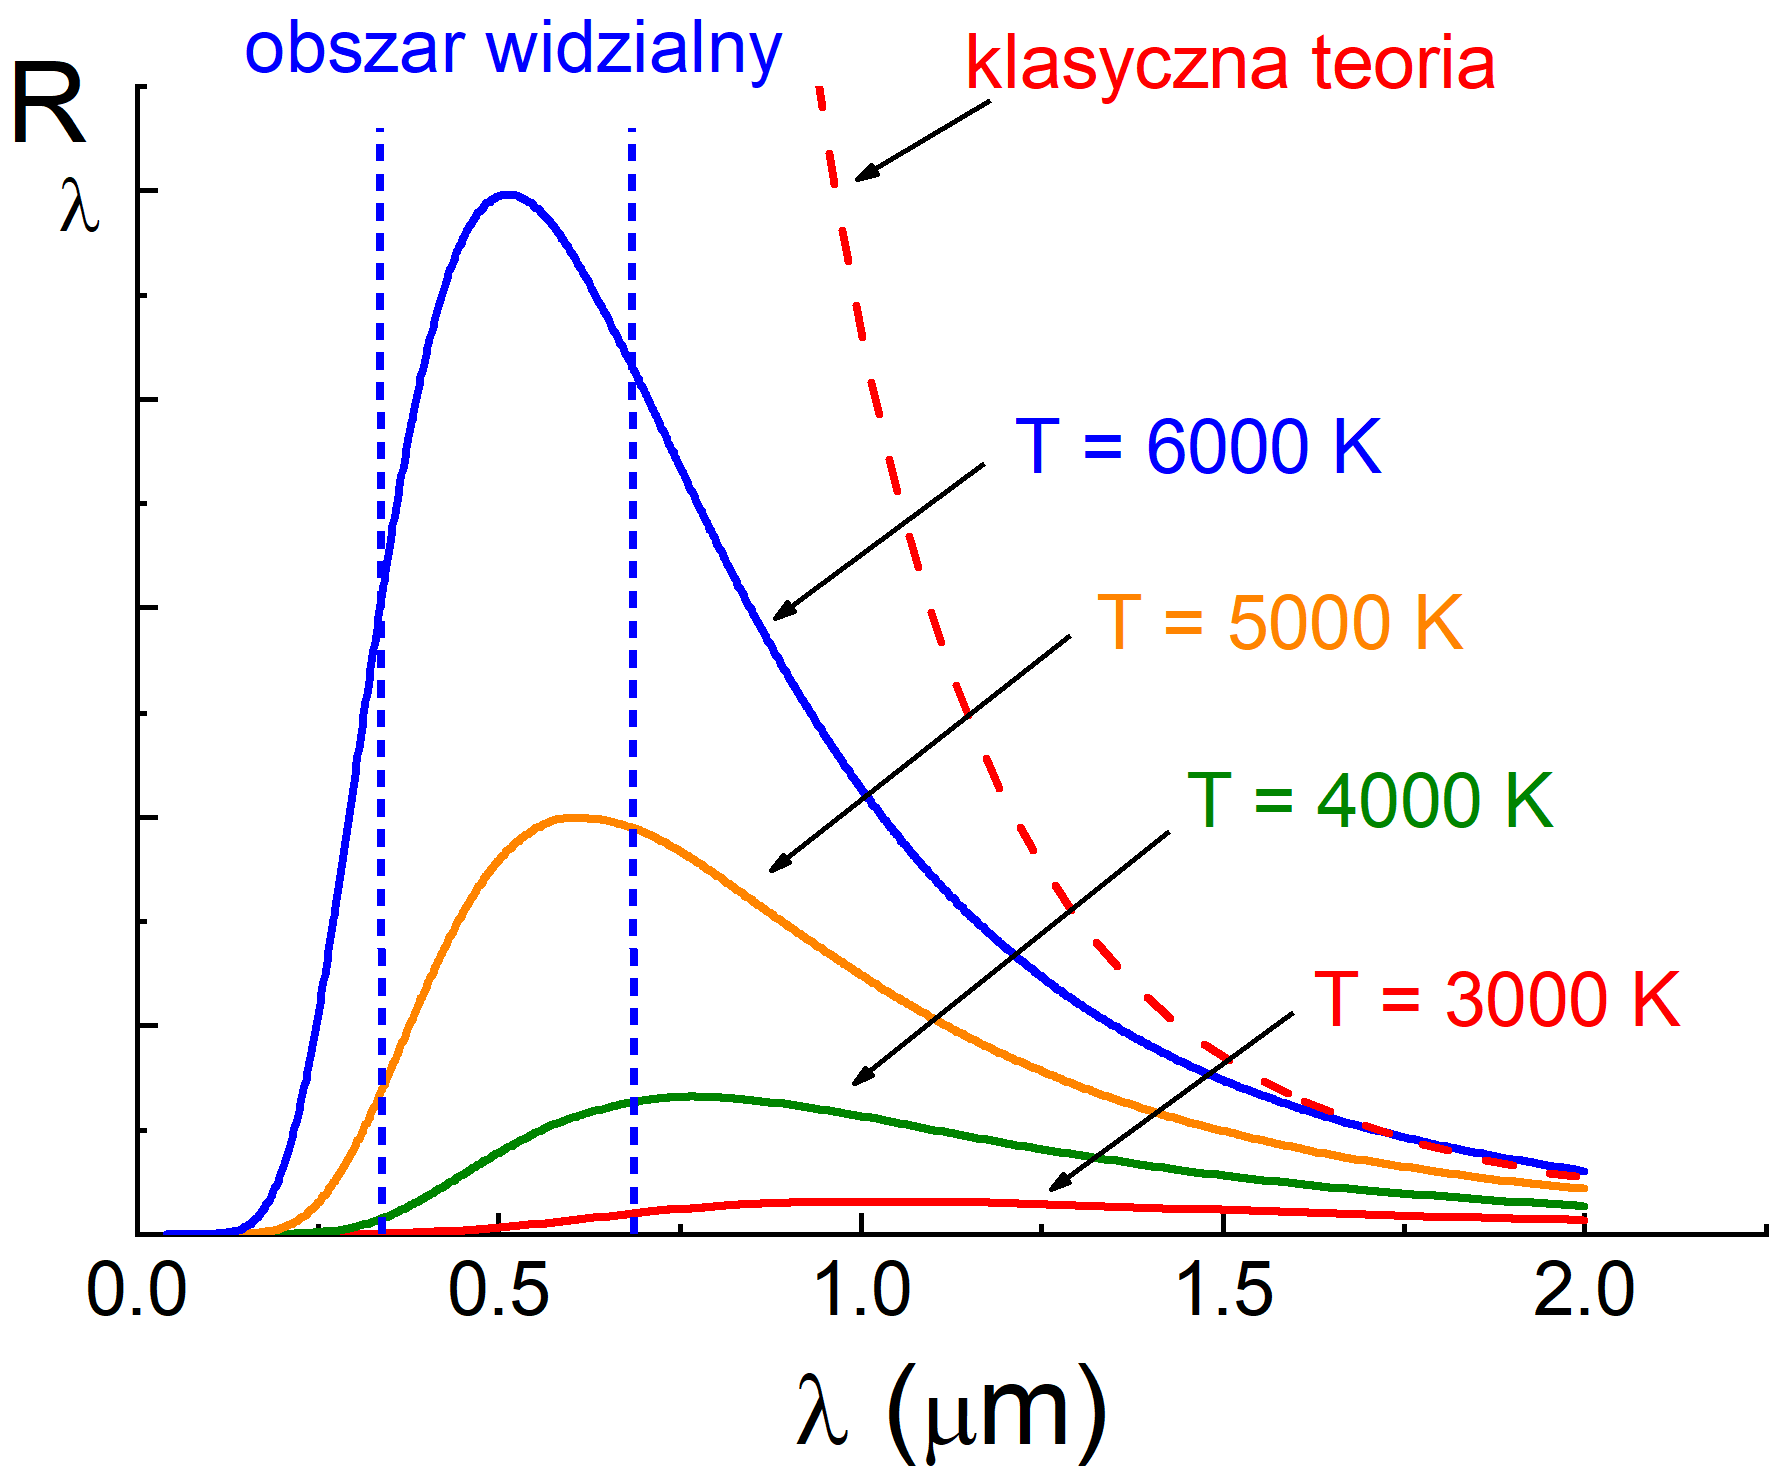
\includegraphics[width=0.5\textwidth]{widmo-promieniowania}
    \caption{Widmo promieniowania ciała doskonale czarnego w wybranych temperaturach. \textit{Źródło: e-Fizyka, AGH}}
    \label{fig:widmo-promieniowania}
\end{figure}

\subsection{Teoria kwantowa Plancka}
W 1900 roku Planck zaproponował, że ciała emitują światło w postaci kwantów ($\epsilon = n\epsilon_0$)
\begin{equation*}
    \bar{\epsilon} = \frac{\sum\limits_{n=0}^{\infty} n\epsilon_0 \exp(-\frac{n\epsilon_0}{kT})}{\sum\limits_{n=0}^{\infty} \exp(-\frac{n\epsilon_0}{kT})} = \cdots = \frac{\epsilon_0}{\exp(\frac{\epsilon_0}{kT}) - 1},
\end{equation*}
gdzie \(\epsilon_0 = h \nu = \frac{h c}{\lambda}\) jest energią jednego kwantu promieniowania.

Z tego wyrażenia Planck otrzymał rozkład promieniowania w funkcji długości fali, który ma postać
\begin{equation*}
    \beta(\lambda, T) = \frac{8\pi hc}{\lambda^5} \cdot \frac{1}{\exp(\frac{hc}{k\lambda T}) - 1},
\end{equation*}
Wzór ten zgadza się z wynikami eksperymentalnymi, eliminując problem ,,katastrofy ultrafioletowej''.

\subsection{Efekt fotoelektryczny}
Efekt fotoelektryczny to zjawisko emisji elektronów z powierzchni metalu pod wpływem padającego na niego światła.

\begin{figure}[H]
    \centering
    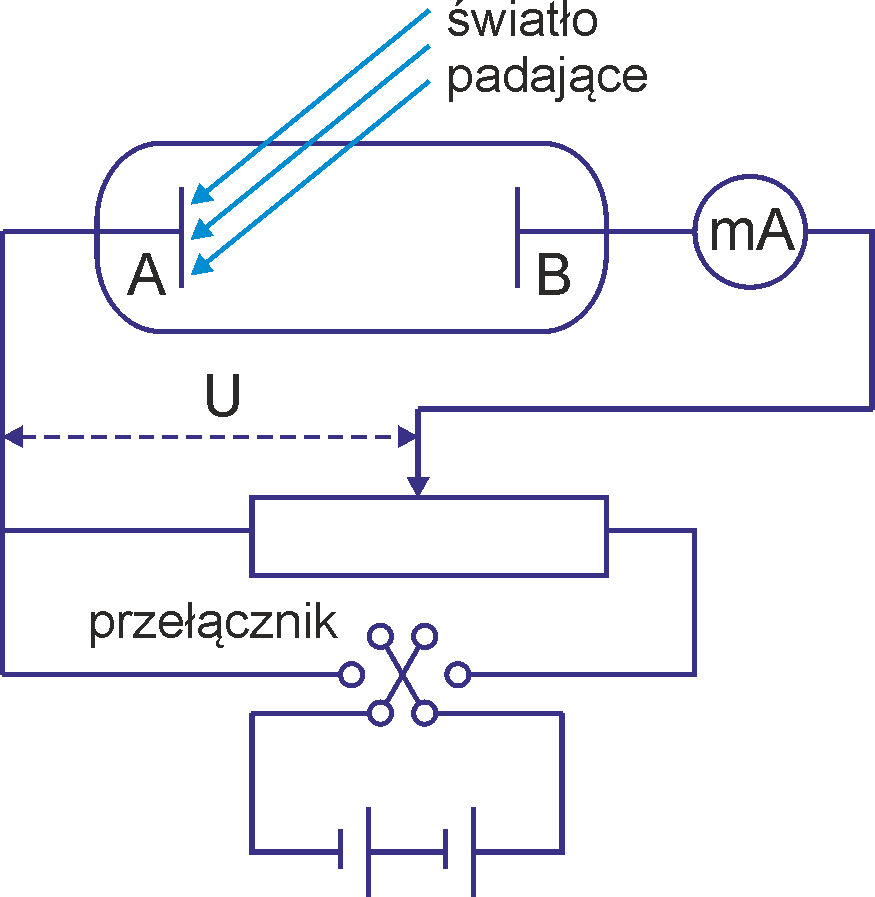
\includegraphics[width=0.5\textwidth]{efekt-fotoelektryczny}
    \caption{Układ do obserwacji zjawiska fotoelektrycznego. \textit{Źródło: e-Fizyka, AGH}}
    \label{fig:efekt-fotoelektryczny}
\end{figure}

W 1900 roku doświadczenia Lenarda wykazały, że energia elektronów zależy od częstotliwości światła, a nie jego intensywności.
Einstein sformułował wzór efektu fotoelektrycznego
\begin{equation*}
    \frac{1}{2} m v_{\max}^2 = h\nu - W,
\end{equation*}
gdzie $W$ to funkcja pracy metalu (zależna od rodzaju metalu).

\subsection{Widma atomowe i model Bohra}
Newton (1660) badał rozszczepienie światła. Melvill (1755) odkrył, że różne pierwiastki mają charakterystyczne linie widmowe. Kirchhoff (1855) zauważył, że widmo zależy od typu atomu i istnieją zarówno widma emisyjne, jak i absorpcyjne.

Balmer (1885) podał wzór:
\begin{equation*}
    \lambda = C \cdot \frac{n^2}{n^2 - 4}.
\end{equation*}

Rydberg sformułował bardziej ogólny wzór:
\begin{equation*}
    \tilde{\nu} = R_H \left( \frac{1}{2^2} - \frac{1}{n^2} \right).
\end{equation*}

\section{Funkcja falowa}

\subsection{Eksperyment z dwoma szczelinami}

Wobrażmy sobie ścianę z dwoma wąskimi otworami oraz drugą równoległą ścianę za nią, która nie ma żadnych otworów.
Teraz wyobraźmy sobie, że osoba strzela kulami we wszystkich kierunkach. Większość kul zatrzymuje się na pierwszej ścianie,
lecz część kul przechodzi przez otwory i trafia na drugą ścianę.
Jakiego obrazu spodziewamy się na drugiej ścianie? Spodziewamy się dwóch kropek, w miejscach odpowiadających otworom na pierwszej ścianie. To też obserwujemy.

\begin{figure}[H]
    \centering
    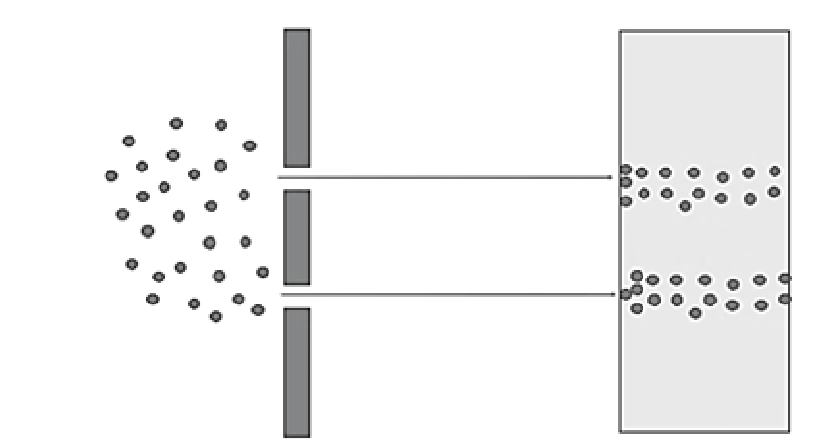
\includegraphics[width=0.5\textwidth]{szczeliny}
    \caption{Eksperyment z dwoma szczelinami. \textit{Źródło: Ranjbar, Vahid. (2023)}}
    \label{fig:szczeliny}
\end{figure}

\subsection{Eksperyment ze światłem}
W roku 1801 Thomas Young przeprowadził podobny eksperyment, ale przepuszczając przez szczeliny światło.
Przez dwie szczeliny przechodziła tak zwana fala płaska, poruszająca się w kierunku ekranu.
W sensie optyki klasycznej albo termodynamiki klasycznej, możemy powiedzieć, że przykładowo światło słoneczne jest taką falą płaską.
Ta fala płaska przechodzi przez szczeliny, a następnie dalej jako fala płaska przemieszcza się w kierunku oddalonego ekranu.

Co zobaczymy na ekranie? Na ekranie zobaczymy coś niespodziewanego - będzie to obraz interferencyjny.
\begin{figure}[H]
    \centering
    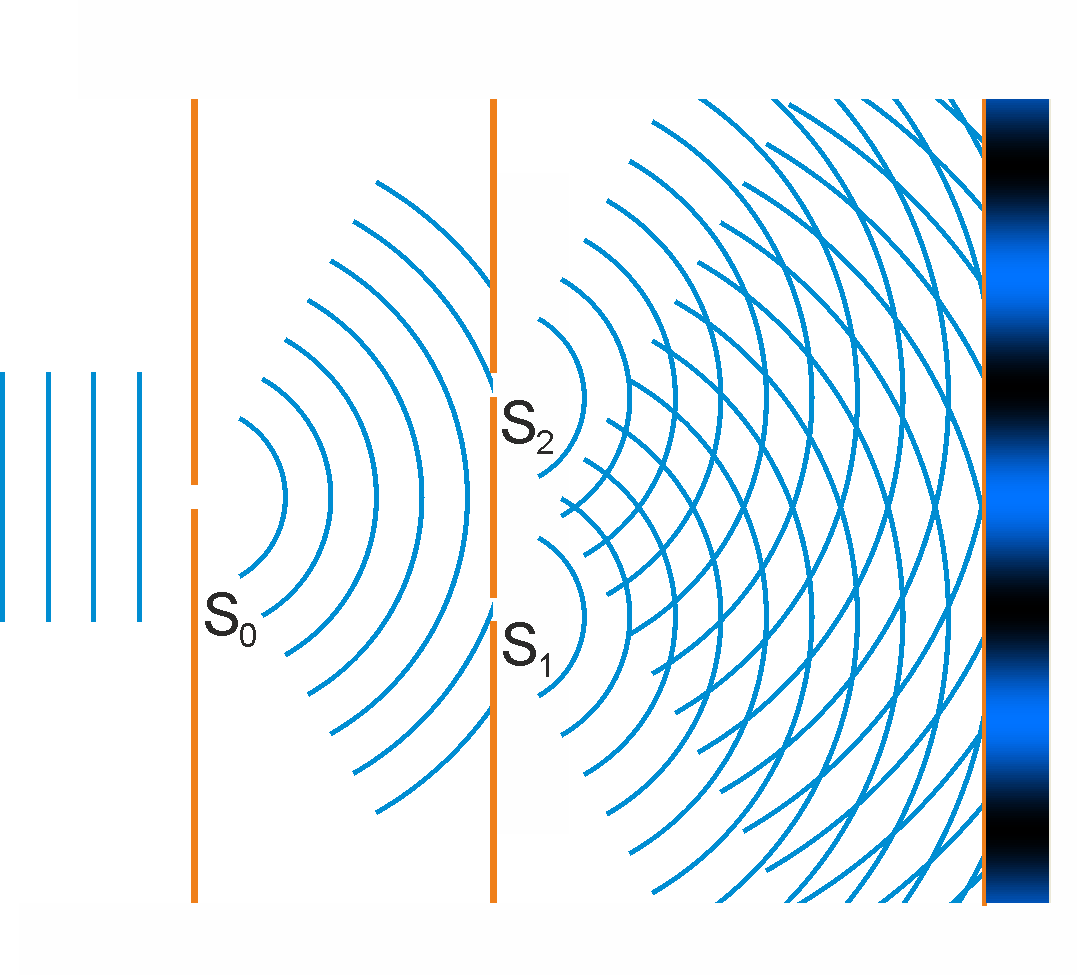
\includegraphics[width=0.5\textwidth]{szczeliny-fale}
    \caption{Eksperyment z dwoma szczelinami. \textit{Źródło: e-Fizyka, AGH}}
    \label{fig:szczeliny-fale}
\end{figure}

Zastanówmy się, w jaki sposób można opisać intensywności światła ukazujące się na ekranie.

Zacznijmy od amplitudy fali (amplitudy światła) - jest to wektor zależny od położenia w przestrzeni oraz czasu:
\begin{equation*}
    A(\bar{r}, t)
\end{equation*}
Intensnywność światła $I$ można zapisać jako kwadrat amplitudy niezależnej od modułu:
\begin{equation*}
    I = |A|^2
\end{equation*}
Następnie pojawia się tak zwana zasada superpozycji. Aby obliczyć amplitudę całkowitą, musimy zsumować amplitudy fal pochodzących z obu szczelin (z obu źródeł):
\begin{equation*}
    \bar{A}(\bar{r}, t) = \bar{A}_1(\bar{r}, t) + \bar{A}_2(\bar{r}, t)
\end{equation*}

Intensywność całkowita będzie przybierać następującą postać:
\begin{equation*}
    I = |A_1|^2 + |A_2|^2 + A_1 A_2^* + A_1^* A_2
\end{equation*}

Człon $A_1 A_2^* + A_1^* A_2$ jest odpowiedzialny za interferencję. Obraz widoczny na ekranie jest spowodowany superpozycją fal pochodzących z obu szczelin.

\subsection{Proste zagadnienie}

Rozważmy najprostsze zagadnienie. W tym zagadnieniu podkreślamy, że odległość między szczelinami $d$ jest mała (dużo mniejsza niż odległość do ekranu $D$).
Na ekranie zaznaczamy pewien punkt $x$ oraz zaznaczamy odległości punktu $x$ od szczelin. Odległość $x$ od szczeliny $1$ wynosi $r_1$, a odległość $x$
od szczeliny $2$ wynosi $r_2$.

\begin{figure}[H]
    \centering
    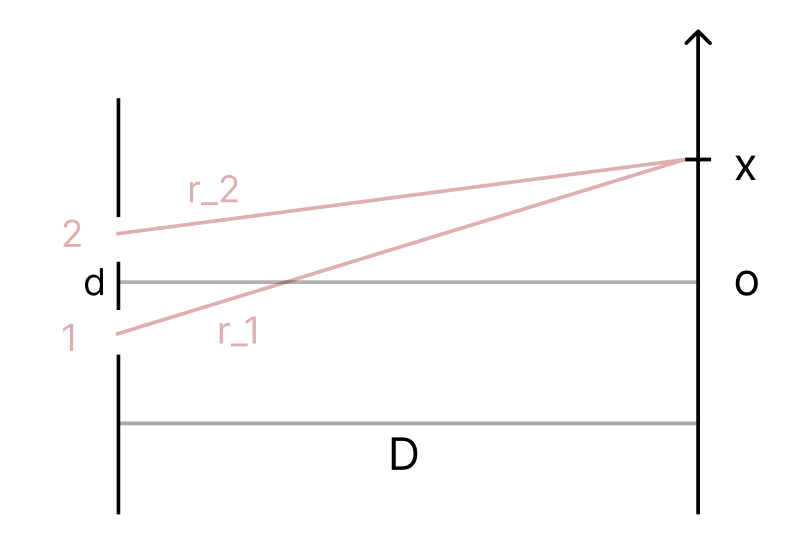
\includegraphics[width=0.5\textwidth]{prosty-eksperyment}
    \caption{Prosty eksperyment.}
    \label{fig:prosty-eksperyment}
\end{figure}

Rozważamy proste fale monochromatyczne, to znaczy amplitudy dla nich mają następującą postać:
\begin{equation*}
    A_1 = a_1 \exp[i(\omega t - \bar{k} \bar{r}_1 + \delta_1)]
\end{equation*}
\begin{equation*}
    A_2 = a_2 \exp[i(\omega t - \bar{k} \bar{r}_2 + \delta_2)]
\end{equation*}

Ponieważ mamy jedno źródło światła, możemy przyjąć, że $a_1 = a_2 = a$ i $\delta_1 = \delta_2 = 0$. 
Symbol $k$ oznacza wektor falowy, który ma kierunek fali. Zapisujemy go jako:
\begin{equation*}
    k = \frac{2\pi}{\lambda}
\end{equation*}
Wersor kierunku fali zapisujemy jako:
\begin{equation*}
    \frac{\bar{k}}{|k|}
\end{equation*}
Przechodzimy do geometrii. Chcemy zrozumieć, jaka będzie intensywność w punkcie $x$ na ekranie.

Wektory $\bar{k}_1$ i $\bar{k}_2$ będą równoległe do siebie, zatem możemy zapisać: $\bar{k}_1 = \bar{k}_2$.


Wyznaczamy $r_1^2$ i $r_2^2$:
\begin{equation*}
    r_1^2 = D^2 + \left(x + \frac{d}{2} \right)^2
\end{equation*}
\begin{equation*}
    r_2^2 = D^2 + \left(x - \frac{d}{2} \right)^2
\end{equation*}
Stąd:
\begin{equation*}
    r_1^2 - r_2^2 = 2xd
\end{equation*}
Ponieważ $r_1$ i $r_2$ są bardzo duże, a różnica między nimi jest mała, możemy zapisać:
\begin{equation*}
    r_1 - r_2 \approx \frac{xd}{D}
\end{equation*}
Intensywność końcowa:
\begin{align*}
    I &= \left(a\cdot e^{i\omega t}\right)^2 \cdot \left[e^{-ikr_1}+e^{-ikr_2}\right]^2 \\
    &= 2 a^2 \left(\cos{\left(kr_1-kr_2\right)}+1\right) \\
    &= 2 a^2 \left(1 + \cos{\left(k(r_1-r_2)\right)}\right) \\
    &= 2 a^2 \left(1 + \cos{\left(\frac{2\pi}{\lambda}\cdot\frac{xd}{D}\right)}\right) = I(x)
\end{align*}

Pytanie - dla jakich $x$ będzie maksymalna intensywność?
Aby znaleźć maksimum, obliczamy pochodną $I(x)$ i przyrównujemy do zera - wartość w zerze będzie albo maksimum, albo minimum.
Chcemy zatem, aby argument cosinusa przyjmował wartość $1$. Będzie to dla $2k\pi$, $k=0,1,2,3,\ldots$. Przyrównując:
\begin{equation*}
    \frac{2\pi}{\lambda} \frac{xd}{D} = 2k\pi
\end{equation*}
Rozwiązując dla $x$ otrzymujemy:
\begin{equation*}
    x_{max} = k \frac{\lambda D}{d}
\end{equation*}
W ten sposób możemy wytłumaczyć obraz interferencyjny - pojawiają się punkty o maksymalnej intensywności
rozłożone wzdłuż osi $x$, a odległość między kolejnymi punktami wynosi $\frac{\lambda D}{d}$.

\section{Stany kwantowe}

\subsection{Eksperyment S-G w interpretacji Feynmana}

Zawartość tego wykładu pochodzi z książki  "'\textit{Feymana wykłady z fizyki} "'. Feyman prowadził te wykłady na początku lat 60 i w głównej mierze zebrały uwagę profesorów gdyż były zbyt ciężkie dla studentów. Przerobimy to w taki sposób, aby to było jasne.
Wprowadźmy oznaczenia. 

\begin{minipage}{0.6 \textwidth}
	\begin{figure}[H]
		\centering
		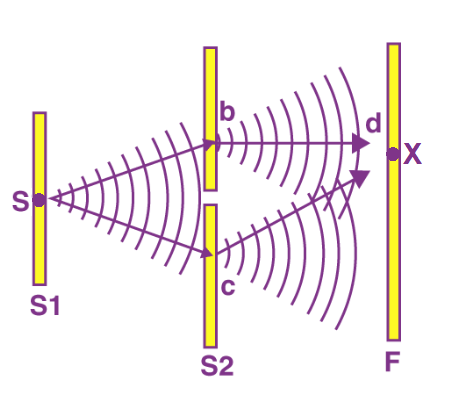
\includegraphics[width=0.5\textwidth]{eksperymentszczelinami}
		\caption{Eksperyment z dwoma szczelinami. \newline \textit{Źródło: Byju's}}
		\label{fig:szczeliny2}
	\end{figure}
\end{minipage}
\begin{minipage}{0.35 \textwidth}
	Prawdopodobieństwo, że elektron ze stanu S przejdzie do stanu X \newline [Stan $X$] $\leftarrow$ [Stan $S$] = $\vert\langle X\vert S\rangle\vert^2$ będziemy nazywać amplitudą.
\end{minipage}

Amplitudę ze stanu $S$ do stanu $X$ możemy w tym przypadku zapisać dwojako, w postaci $\langle X\vert1\rangle, \langle 1\vert S\rangle$ jako przejścia ze stanu $S$ do stanu $1$ a następnie ze stanu $1$ do stanu $X$, oraz analogicznie w postaci $\langle X\vert2\rangle , \langle 2\vert S\rangle$. Przepiszemy korzystając z tych oznaczeń zasadę superpozycji. Jeżeli chcemy przejść ze stanu $S$ do stanu $X$ to będziemy to zapisywać jako sumę amplitud $\langle X\vert S\rangle = \langle X\vert1\rangle\langle 1\vert S\rangle + \langle X\vert2\rangle \langle 2\vert S\rangle$. Jeżeli chcemy zapisać prawdopodobieństwo to musimy obliczyć z tego moduł do kwadratu i obliczyć to wszystko w liczbach zespolonych $\vert\langle X\vert S\rangle \vert^2 = \vert[...]\vert^2$. 
\textbf{Pytanie} co oznacza superpozycja? Jeżeli chcemy obliczyć amplitudę to jest to suma poszczególnych amplitud. Amplituda $S$ do $Z$ jest superpozycją przejścia przez szczeliny.
\subsection{Urządzenie S-G dla atomów ze spinem 1}
\begin{minipage}{0.2 \textwidth}
	\vspace{11pt}
	Spin oznaczamy
\end{minipage}
\begin{minipage}{0.11 \textwidth}
    \begingroup
    \hfuzz=1000pt
	\begin{equation*}
		X_{\beta} = 
		\begin{cases}
			+1 \\
			0 \hspace{20pt} \leftarrow \text{ trzy rodzaje kwantowe.} \\
			-1 \\
		\end{cases}
	\end{equation*}
    \endgroup
\end{minipage}
\begin{figure}[H]
	\centering
	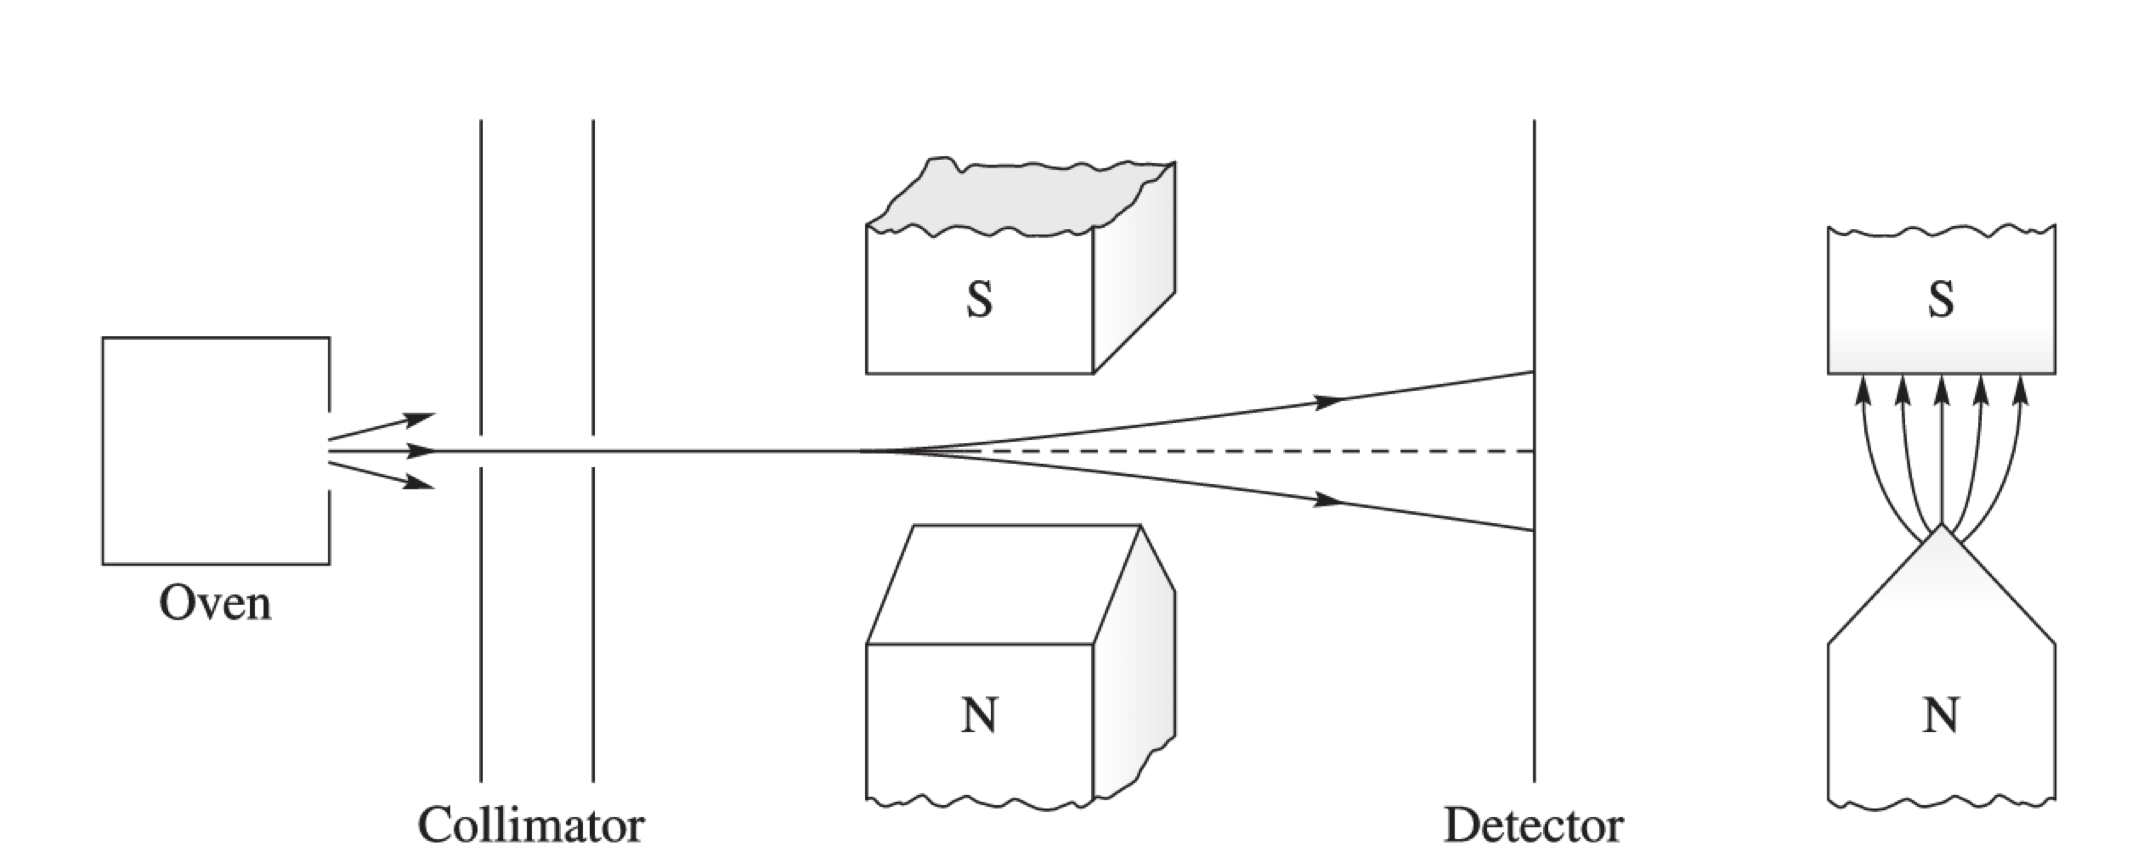
\includegraphics[width=0.6\textwidth]{urzadzeniesg}
	\caption{Urządzenie Sterna-Gerlacha. \textit{Źródło: PennState ESM}}
	\label{fig:urzSG}
\end{figure}
\begin{figure}[H]
	\centering
	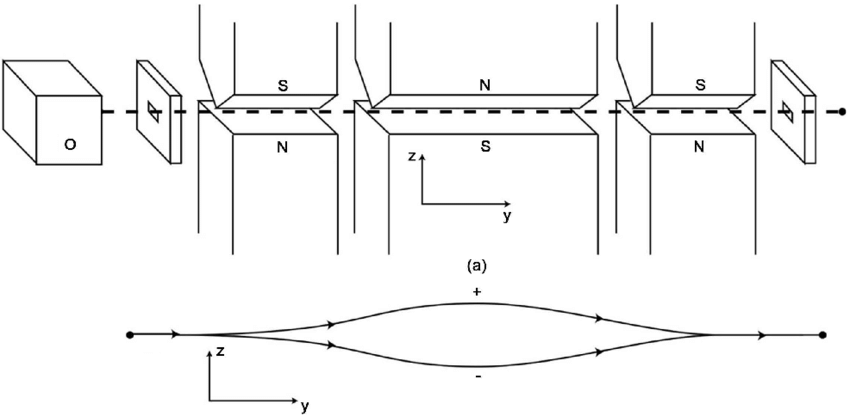
\includegraphics[width=0.8\textwidth]{urzadzeniesgmod.png}
	\caption{Modyfikacja urządzenia Sterna-Gerlacha. \textit{Źródło: ResearchGate}}
	\label{fig:urzSGmod}
\end{figure}
Dlaczego tak robimy? Ponieważ dzięki zmodyfikowaniu urządzenia S-G nasze atomy będą podążały jak na rysunku powyżej do jednego punktu. I to będzie nasze modyfikowane urządzenie S-G o którym dalej będziemy mówić. Następnie możemy rozważyć kolejny schemat. Możemy wstawić płytkę przez którą nie mogą przechodzić atomy, więc na końcu będziemy mieli tylko atomy nie zablokowane.

\begin{minipage}{0.5 \textwidth}
	\begin{figure}[H]
		\centering
		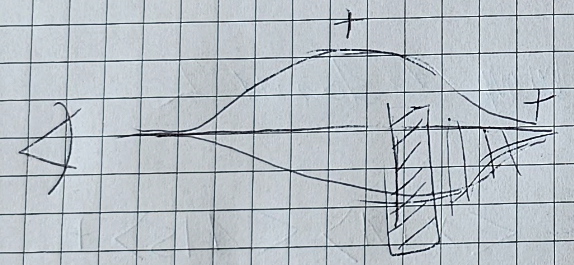
\includegraphics[width=0.8\textwidth]{urzadzeniesgblok}
		\caption{Zablokowane atomy poza  "'$+$ "'}
		\label{fig:urzSGblok}
	\end{figure}
\end{minipage}
\begin{minipage}{0.05 \textwidth}
	\vspace{-20pt}
	\begin{equation*}
		\hspace{-30pt}
		\left\{\begin{array}{lr}
			+ \\
			0 \hspace{3pt} \vert \\
			- \vert
		\end{array}\right\}
	\end{equation*}
\end{minipage}
\begin{minipage}{0.45 \textwidth}
	Będziemy podpisywać modyfikacje z zablokowanymi  "'$0$ "' oraz  "'$-$ "' jako  "'$+S$ "', analogicznie  "'$0S$ "' oraz  "'$-S$ "'
\end{minipage}


\begin{minipage}{0.6 \textwidth}
	\begin{figure}[H]
		\centering
		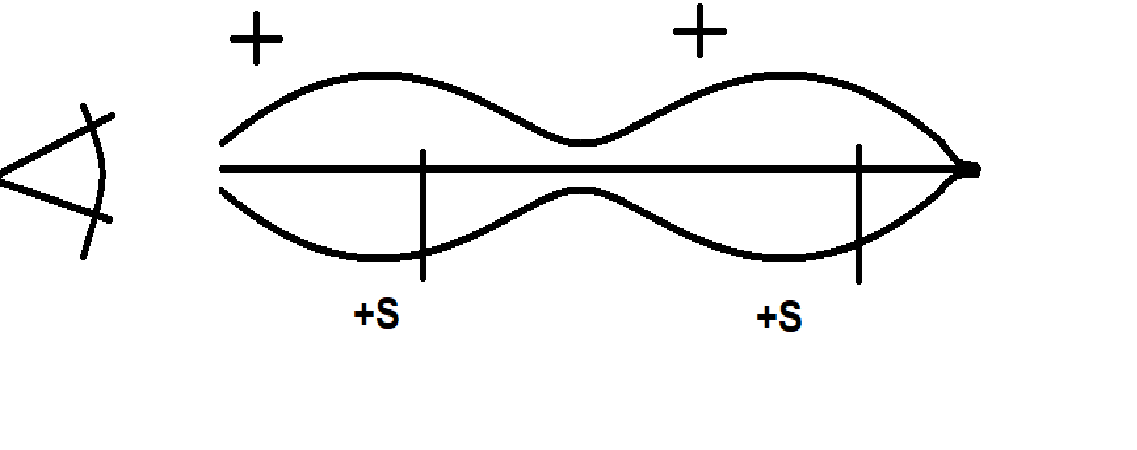
\includegraphics[width=0.6\textwidth]{urzsgblok2}
		\caption{Zablokowane atomy poza  "'$+$ "' dwa razy}
		\label{fig:urzSGblok2}
	\end{figure}
\end{minipage}
\begin{minipage}{0.5 \textwidth}
	\vspace{-40pt}
	$\langle +S \vert +S \rangle = 1$, dlatego że wszystkie atomy przejdą najpierw górnym, a potem będą tylko i wyłącznie dostępne atomy z plusem, więc wszystkie atomy znowu przejdą, więc zawsze wychodzi $1$. Jest to postulat.
\end{minipage}


\begin{minipage}{0.6 \textwidth}
	\begin{figure}[H]
		\centering
		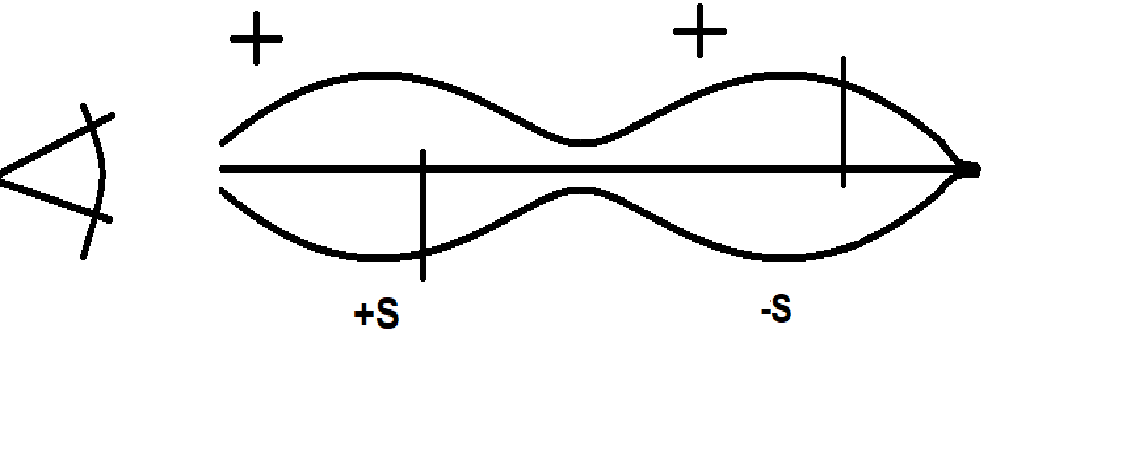
\includegraphics[width=0.6\textwidth]{urzsgblok3}
		\caption{Zablokowane atomy raz poza  "'$+$ "' i raz poza  "'$-$ "'}
		\label{fig:urzSGblok3}
	\end{figure}
\end{minipage}
\begin{minipage}{0.5 \textwidth}
	\vspace{-40pt}
	$\langle -S \vert +S \rangle = 0$
\end{minipage}
\newpage
Możemy w taki sposób wymienić różne stany początkowe i końcowe i możemy stworzyć tabelę
\begin{table}[ht]
	\centering
	\begin{tabular}[t]{c|c|c|c}
		& $+S$ & $0S$ & $-S$\\
		\hline
		$+S$ & $1$ & $0$ & $0$ \\
		\hline
		$0S$ & $0$ & $1$ & $0$ \\
		\hline
		$-S$ & $0$ & $0$ & $1$ \\
	\end{tabular}
	\label{tab:stany}
\end{table}

Następnie rozważmy sytuacje gdzie mamy  "'pokręcone "' urządzenie S-G. Niech pierwsze urządzenie będzie się nazywało urządzeniem "'$S$"' a drugie urządzeniem "'$T$"'

\begin{figure}[H]
	\centering
	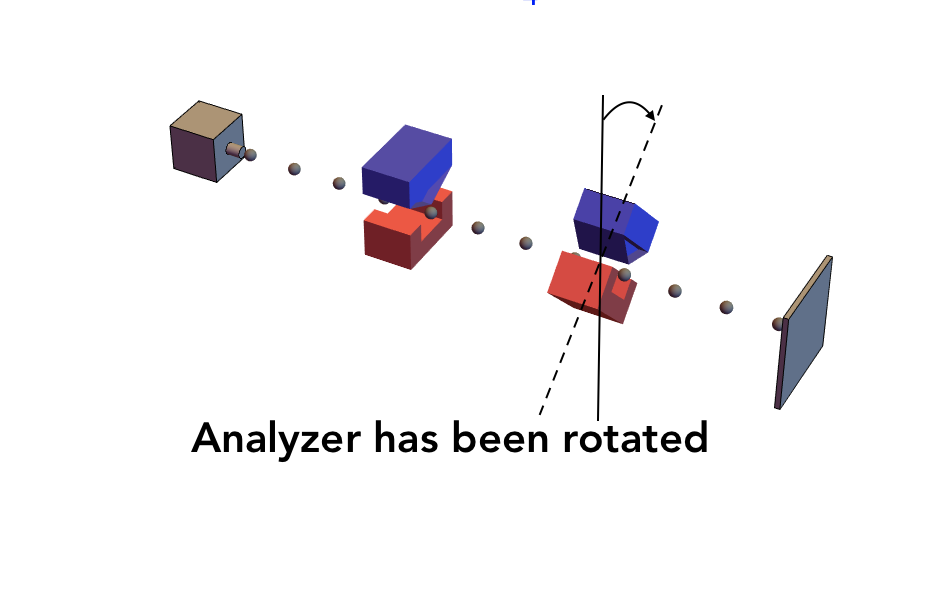
\includegraphics[width=0.8\textwidth]{SGArot}
	\caption{Obrócone urządzenie S-G, \textit{Źródło: Deepnote}}
	\label{fig:SGArot}
\end{figure}

Jeżeli mamy na początku stan "'$+S$ "'  a następnie przechodzimy przez urządzenie ze stanem "'$-T$ "' to co będziemy mieli? 


\begin{equation*}
	\left\{\begin{array}{lr}
		+ \\
		0 \hspace{3pt} \vert \\
		- \vert
	\end{array}\right\} 
	\left\{\begin{array}{lr}
		+ \vert \\
		0 \hspace{3pt} \vert \\
		- 
	\end{array}\right\}
	\neq 0 \text{,} \hspace{10pt}  \langle-T \vert +S\rangle \neq 0
\end{equation*}
Jeżeli chcemy obliczyć prawdopodobieństwo przejścia ze stanu "'$+S$ "' do stanu "'$+T$ "' to możemy to obliczyć następująco
\begin{equation*}
	\left| \langle\ +T\vert+S \rangle \right|^2 = \langle\ +T\vert+S \rangle \langle\ +T\vert+S \rangle^*
\end{equation*}
Gdy prowadzimy kilka doświadczeń w których będziemy mieli początek w "' $+S$ "' a następnie przejdziemy przez urządzenia "'$+T$ "' i  "'$0T$ "' oraz "'$0T$ "', to prawdopodobieństwo że cząstka przejdzie końcowo przez którekolwiek z urządzeń "'$T$ "' jest jedynką.

\begin{equation*}
	\langle\ +T\vert+S \rangle \langle\ +T\vert+S \rangle^* + \langle\ 0T\vert+S \rangle \langle\ 0T\vert+S \rangle^* +\langle\ -T\vert+S \rangle \langle\ -T\vert+S \rangle^* =1
\end{equation*}
Następnie rozważmy schemat eksperymentu gdzie najpierw mamy urządzenie "' $0S$ "', następnie "' $0T$ "' a końcowo "' $+S$ "'. Wtedy amplituda $\langle\ +S\vert0T \rangle \langle\ 0T\vert0S \rangle^*$ będzie następująca
\begin{equation*}
	\frac{p_2}{p_1} = \frac{\left|\langle\ +S\vert0T \rangle \langle\ 0T\vert0S \rangle\right|^2}{\left|\langle\ 0S\vert0T \rangle \langle\ 0T\vert0S \rangle\right|^2} = \frac{\left|\langle\ +S\vert0T \rangle\right|^2}{\left|\langle\ 0S\vert0T \rangle\right|^2}
\end{equation*}
Rozważmy trzy schematy eksperymentu gdzie $N$ cząstek będzie przechodzić z urządzenia "' $S$ "' do urządzenia "' $T$ "' i znowu do "' $S$ "'.
\begin{equation*}
	\hspace{-50pt} (1)
	\left\{\begin{array}{lr}
		+ \\
		0 \hspace{3pt} \vert \\
		- \vert
	\end{array}\right\} 
	\xrightarrow[N]{}
	\left\{\begin{array}{lr}
		+  \\
		0  \\
		- 
	\end{array}\right\}
	\xrightarrow[N]{}
	\left\{\begin{array}{lr}
		+  \\
		0 \hspace{3pt} \vert \\
		- \vert
	\end{array}\right\}
	\xrightarrow[N]{} \text{To urządzenie nic nie zmienia}
\end{equation*}

\begin{equation*}
	\hspace{-140pt} (2)
	\left\{\begin{array}{lr}
		+ \\
		0 \hspace{3pt} \vert \\
		- \vert
	\end{array}\right\} 
	\xrightarrow[N]{}
	\left\{\begin{array}{lr}
		+  \\
		0  \\
		- 
	\end{array}\right\}
	\xrightarrow[N]{}
	\left\{\begin{array}{lr}
		+ \vert \\
		0  \\
		- \vert
	\end{array}\right\}
	\xrightarrow[0]{} \text{Zero cząstek}
\end{equation*}

\begin{equation*} (3)
	\left\{\begin{array}{lr}
		+ \\
		0 \hspace{3pt} \vert \\
		- \vert
	\end{array}\right\} 
	\xrightarrow[N]{}
	\left\{\begin{array}{lr}
		+ \vert \\
		0 \hspace{3pt} \vert \\
		- 
	\end{array}\right\}
	\xrightarrow[N]{}
	\left\{\begin{array}{lr}
		+ \vert \\
		0  \\
		- \vert
	\end{array}\right\}
	\xrightarrow[\beta\alpha N]{\alpha \leq 1, \beta \leq 1} \text{Tu przechodzi tylko część cząstek}
\end{equation*}
W przypadku eksperymentu $(3)$, urządzenie "' $T$ "' jest bardziej restrykcyjne niż w przypadku eksperymentu $(2)$, jednak mimo tego końcowo przechodzi niezerowa ilość cząstek. To jest przykład zupełnie kwantowy.
Można to zrozumieć analogicznie w kontekście wektorów, przy standardowym rzutowaniu najpierw na oś $OY$ a następnie na $OX$ zawsze kończymy w zerze, jednak gdybyśmy mieli dodatkowe osie $OY'$ oraz $OX'$ i rzutowali po kolei $OY \rightarrow OY' \rightarrow OX$ to pomimo nałożenia dodatkowego restrykcyjnego rzutowania otrzymujemy wynik niezerowy.
Ze schematu drugiego widzimy
\begin{equation*}
	a = 0 = \left|\langle\ 0S \vert +T \rangle \right| \left|\langle\ +T \vert +S \rangle \right| + 
	\left|\langle\ 0S \vert 0T \rangle \right| \left|\langle\ 0T \vert +S \rangle \right| + 
	\left|\langle\ 0S \vert -T \rangle \right| \left|\langle\ -T \vert +S \rangle \right|
\end{equation*}
Amplitudy mamy interferencyjne i w rezultacie mamy 0. Ze schematu pierwszego natomiast
\begin{equation*}
	a = 1 = \left|\langle\ +S \vert +T \rangle \right| \left|\langle\ +T \vert +S \rangle \right| + 
	\left|\langle\ +S \vert 0T \rangle \right| \left|\langle\ 0T \vert +S \rangle \right| + 
	\left|\langle\ +S \vert -T \rangle \right| \left|\langle\ -T \vert +S \rangle \right|
\end{equation*}
\subsection{Bazy}
Niech $\vert +T \rangle = \vert 1 \rangle$, $\vert 0T \rangle = \vert 2 \rangle$, $\vert -T \rangle = \vert 3 \rangle$. Wtedy możemy zapisać amplitudę $a$ jako sumę
\begin{equation*}
	a = \sum_{i = 1}^3 \langle\ +S \vert i \rangle \langle\ i \vert +S \rangle = 1 = \langle\ +S \vert +S \rangle
\end{equation*}
Dzięki temu możemy zapisać niezależnie od tego jakie mamy urządzenia. Dla schematu z urządzeniami $S$ oraz $R$ mamy
\begin{equation*}
	\left\{\begin{array}{lr}
		+ \\
		0 \hspace{3pt} \vert \\
		- \vert
	\end{array}\right\} 
	\left\{\begin{array}{lr}
		+ \\
		0 \hspace{3pt} \vert \\
		- \vert
	\end{array}\right\} 
	\iff a =  \langle\ +R \vert +S \rangle \langle\ = \sum_{i = 1}^3 \langle\ +R \vert i \rangle \langle\ i \vert +S \rangle
\end{equation*}
Zapiszmy $\vert +R \rangle = \vert \chi \rangle$, $\vert +S \rangle = \vert \phi \rangle$, i wtedy mamy zapis które wszędzie można spotkać w mechanice kwantowej
\begin{equation*}
	\langle\ \chi \vert \phi \rangle = \sum_{i} \langle\ \chi \vert i \rangle \langle\ i \vert \phi \rangle
\end{equation*}
Możemy z tego zapisać kilka reguł (pod warunkiem że $i \neq j$)
\begin{equation*}
	\begin{split}
		\langle\ i \vert i \rangle &= 1 \\
		\langle\ i \vert j \rangle &= 1
	\end{split}
\end{equation*}
Przepiszmy równanie które już wcześniej wyliczyliśmy w tym rozdziale.
\begin{equation*}
	\langle\ +T\vert+S \rangle \langle\ +T\vert+S \rangle^* + \langle\ 0T\vert+S \rangle \langle\ 0T\vert+S \rangle^* +\langle\ -T\vert+S \rangle \langle\ -T\vert+S \rangle^* =1.
\end{equation*}
Łącząc je z równaniem dające wynik amplitudy $a = 1$ dostajemy zależności
\begin{equation*}
	\begin{split}
		\langle\ +S \vert +T \rangle &= \langle\ +T \vert +S \rangle^* \\
		\langle\ +S \vert 0T \rangle &= \langle\ 0T \vert +S \rangle^* \\
		\langle\ +S \vert -T \rangle &= \langle\ -T \vert +S \rangle^* 
	\end{split}
\end{equation*}
Daje nam to kolejną regułę
\begin{equation*}
	\langle\ \chi \vert \phi \rangle = \langle\ \phi \vert \chi \rangle^*
\end{equation*}
\subsection{Operatory}
Amplitudę że przejdziemy ze stanu $+S$ do $0R$ możemy zapisać jako
\begin{equation*}
	a = \langle\ 0R \vert \dots \rangle \langle\ \dots \vert \dots \rangle \dots \langle\ \dots \vert \dots \rangle \langle\ \dots \vert +S \rangle  = \langle\ 0R \vert A \vert +S \rangle 
\end{equation*}
gdzie $A$ to są różne operacje związane ze zbiorem urządzeń. Przez $\hat{A}$ będziemy oznaczać operator generalny.
Możemy też zapisać macierz operatora $\hat{A}$. Niech $\vert +S \rangle$, $\vert 0S \rangle$, $\vert -S \rangle$ będą stanami naszej bazy. Wtedy mamy
\begin{table}[ht]
	\centering
	\begin{tabular}[t]{c|c|c|c}
		& $+$ & $0$ & $-$\\
		\hline
		$+$ & $\langle\ + \vert \hat{A} \vert + \rangle $ & $\langle\ + \vert \hat{A} \vert 0 \rangle $ & $\langle\ + \vert \hat{A} \vert - \rangle $ \\
		\hline
		$0$ & $\langle\ 0 \vert \hat{A} \vert + \rangle $ & $\langle\ 0 \vert \hat{A} \vert 0 \rangle $ & $\langle\ 0 \vert \hat{A} \vert - \rangle $ \\
		\hline
		$-$ & $\langle\ - \vert \hat{A} \vert + \rangle $ & $\langle\ - \vert \hat{A} \vert 0 \rangle $ & $\langle\ - \vert \hat{A} \vert - \rangle $ \\
	\end{tabular}
	\label{tab:macierzoperatora}
\end{table}

Powyższe nazywamy macierzą operatora $\hat{A}$ w bazie takiej jak wyżej podanej. Dajemy też czapkę nad operatorem aby zawsze było wiadomo że chodzi nam o operator, ale nie zawsze trzeba to pisać. Operator nigdy nie jest zależny od bazy ale macierz operatora zawsze jest w jakiejś bazie.
Następnie wyprowadźmy parę własności.
\begin{equation*}
	\left\{\begin{array}{lr}
		+ \\
		0  \\
		- 
	\end{array}\right\}_{S} 
	\left\{\begin{array}{lr}
		+ \\
		0 \\
		- 
	\end{array}\right\}_{T_i}
	\hat{A}
	\left\{\begin{array}{lr}
		+ \\
		0  \\
		- 
	\end{array}\right\}_{T_j} 
	\left\{\begin{array}{lr}
		+ \vert \\
		0 \\
		- \vert
	\end{array}\right\}_{R}
	=
	\left\{\begin{array}{lr}
		+ \\
		0  \\
		- 
	\end{array}\right\}_{S} 
	\hat{A}
	\left\{\begin{array}{lr}
		+ \vert \\
		0 \\
		- \vert
	\end{array}\right\}_{R}
\end{equation*}
Możemy powiedzieć że weźmiemy bazę tego urządzenia $T$ i wtedy możemy to zapisać inaczej jako

\begin{equation*}
	\sum_{ij} \langle\ 0R \vert j \rangle \langle\ j \vert A \vert i \rangle \langle\ i \vert +S \rangle = \langle\ OR \vert A \vert +S \rangle
\end{equation*}
Inaczej możemy zapisać, uogólniając tą regułę, że 
\begin{equation*}
	\langle\ \chi \vert A \vert \phi \rangle = \sum_{ij} \langle\ \chi \vert j \rangle \langle\ j \vert A \vert i \rangle \langle\ i \vert \phi \rangle
\end{equation*}
Niech urządzenie $C$ to urządzenie $B$ które stoi tuż po urządzeniu $A$.
\begin{equation*}
	\{C\} = \{A\} \{B\} = \{A\} \left\{\begin{array}{lr}
		+ \\
		0 \\
		- 
	\end{array}\right\}_{T} \{B\}
\end{equation*}
Przez to możemy zapisać
\begin{equation*}
	\langle\ j \vert C \vert i \rangle = \sum_{ij} \langle\ j \vert B \vert k \rangle \langle\ k \vert A \vert i \rangle
\end{equation*}
A także zapisać to jak mnożenie macierzowe
\begin{equation*}
	\hat{C} = \hat{A} \cdot \hat{B} \rightarrow C = A \cdot B
\end{equation*}
\subsection{Przekształcenia bazy}
Powiedzmy że $\hat{A}$ - operator. Mamy też dwie dowolne ortonormalne bazy $\{1\}$ oraz $\{2\}$. Pytanie jest takie: powiedzmy że mamy operator $\langle\ i_1 \vert \hat{A} \vert j_1 \rangle$. W jaki sposób będą wyglądały elementy macierzowe operatora $\hat{A}$ w bazie $\{2\}$? Do tego potrzebujemy przekształcenia bazy.
\begin{equation*}
	\vert i_2 \rangle = \sum_{j_1} D_{i_2 j_1} \vert j_1 \rangle 
\end{equation*}
Wprowadźmy też tutaj nazewnictwo $\langle j \vert$ - stan "bra", $\vert i \rangle$ - stan "kiet".
Jeżeli ${\vert i \rangle}$ - baza, a $\vert \phi \rangle$ - stan, i jeżeli z tych mamy amplitudy $\langle i \vert \phi \rangle = C_i$, $\langle j \vert \phi \rangle = C_j$, to wtedy możemy powiedzieć że
\begin{equation*}
	\vert \phi \rangle = \sum_{i} C_i \vert i \rangle 
\end{equation*}
Gdzie $C_i$ to amplitudy lub współczynniki. Możemy też pisać
\begin{equation*}
	\vert \chi \rangle = \begin{pmatrix} c_1 \\ c_2 \\ c_3 \end{pmatrix} = c_1 \vert 1 \rangle + c_2 \vert 2 \rangle + c_3 \vert 3 \rangle 
\end{equation*}
W takiej sytuacji piszemy że jakieś $\chi$ jest wektorem, jakimś rozłożeniem w bazie przestrzeni którą mamy. 
Niech też wektor "kiet" będzie 
\begin{equation*}
	\vert \chi \rangle = \sum_i \vert i \rangle D_i.
\end{equation*}
Wtedy wektor "bra" możemy zapisać następująco
\begin{equation*}
	\langle \chi \vert = \sum_j \rangle D_i^* \langle i \vert.
\end{equation*}
Dlaczego tak piszemy? Zobaczmy że dzięki naszemu zapisowi mamy poniższe
\begin{equation*}
	\langle \chi \vert \chi \rangle =  1 = \sum_{ij} \langle i \vert j \rangle D_i^* D_j.
\end{equation*}
Wtedy jeżeli mamy policzyć amplitudę $\langle \chi \vert \phi \rangle$ mamy
\begin{equation*}
	\langle \chi \vert \chi \rangle = \sum_{ij} D_j^* \langle j \vert i \rangle C_i = \sum_i D_i^* C_i
\end{equation*}
I w taki sposób będziemy obliczać powyższą amplitudę z przekształceniem bazy. Zapiszmy też
\begin{equation*}
	\langle\ i_2 \vert A \vert j_2 \rangle = \left(\sum_k D_{il}^* \langle l_1 \vert  \right) A \left(\sum_k D_{jk} \vert k_1 \rangle \right) = \sum_{lk} D_{il}^* D_{jk} \langle l_1 \vert A \vert k_1 \rangle
\end{equation*}
Nie wszystkie bazy są takie same, każde zagadnienie potrzebuje odpowiedniej (wygodnej) bazy i będziemy się tego uczyć.
\subsection{Równanie Schrödingera}
Czas wpływa na ewolucje dowolnego układu kwantowego. $U(t_2, t_1)$ - operator ewolucji.
\begin{equation*}
	\langle \chi \vert \hat{U}(t_2, t_1)\vert \phi \rangle - \text{amplituda}, \vert \phi \rangle \xrightarrow{t_1 \rightarrow t_2} \vert \chi \rangle
\end{equation*}
\begin{equation*}
	\langle i \vert \hat{U}(t_2, t_1)\vert j \rangle, \text{ gdzie $t_2$ - czas końcowy, $t_1$ - czas początkowy}
\end{equation*}
Mówimy, że operator ewolucji posiada własność
\begin{equation*}
	U(t_3, t_1) = U(t_3,t_2)U(t_2,t_1) \leftarrow \text{ postulat}
\end{equation*}
Dla $\delta t$ małego czasu możemy wypisywać, że stan układu w czasie
\begin{equation*}
	\vert \psi (t + \Delta t) \rangle = U(t+\Delta t, t\vert \psi(t) \rangle )
\end{equation*}
Możemy obliczyć współczynniki amplitudy dla stanu bazowego i
\begin{equation*}
	C_i(t+\Delta t) \leftarrow \langle i \vert \psi(t + \Delta t) \rangle = \langle i \vert U(t + \Delta t, t) \vert \psi(t)\rangle = \sum_j \langle i \vert U(t + \Delta t, t) \vert j \rangle \langle j \vert \psi(t) \rangle \rightarrow C_j(t)
\end{equation*}
\begin{equation*}
	C_j(t+\Delta t) = \sum_j U_{ij}(t + \Delta t, t) C_j(t)
\end{equation*}
Mamy też postulat
\begin{equation*}
	U_{ij}(t + \Delta t, t) = \delta_{ij} - \frac{i}{\hbar}H_{ij}(t)\Delta t
\end{equation*}
Gdzie $\frac{i}{\hbar}H_{ij}(t)$ jest wygodnym elementem macierzowym i korzystnym później. Gdy mamy operator $U_{ij}(t, t)$ to nic się nie zmienia [trywialne]. Wykonajmy teraz kilka przekształceń
\begin{equation*}
	\begin{split}
		C_j(t + \Delta t) &= \sum_j (\delta_{ij} - \frac{i}{\hbar}H_{ij}(t)\Delta t)C_J(t)\\
		C_j(t + \Delta t) &= C_j(t) - \frac{i}{\hbar}\Delta t \sum_j H_{ij} H(t) C_j(t) \\
		\frac{C_j(t + \Delta t) - C_j(t)}{\Delta t} &= - \frac{i}{\hbar} \sum_j H_{ij}(t) C_j(t)
	\end{split}
\end{equation*}
Korzystając teraz z zapisu $\dot{c}_i(t)$ - pochodna po czasie, zapiszmy
\begin{equation*}
	i\hbar \dot{c}_i(t) = \sum_j H_{ij}(t) C_j(t)
\end{equation*}
Niech także
\begin{equation*}
	\overrightarrow{c}(t) = \begin{pmatrix} c_1(t) \\ c_2(t) \\ \vdots \end{pmatrix}
\end{equation*}
Wtedy możemy zapisać
\begin{equation*}
	i\hbar \overrightarrow{c}(t) =  \hat{H}(t) \hat{C}(t)
\end{equation*}
\textbf{Pytanie} czy skoro H jest zależne od czasu tutaj, to później też takie będzie czy raczej stałe? To będzie zależeć od zagadnienia, ale łatwiej jest jak nie ma tej zależności.
Wiemy też że cząstka musi być w jakimś stanie, więc
\begin{equation*}
	\sum_i \vert C_i(t)\vert^2 = 1.
\end{equation*}

\textbf{Pytanie} skoro c jest niewiadoma to czy H jest znane? H jest znane (sztuka rozsądnego zgadywania) i takie aby równanie było poprawne.

\textbf{Pytanie} czy i to jest stan z bazy? Tak
\subsection{Przykład: Ewolucja atomu z 2 stanami w polu laserowym}
Powiedzmy, że mamy atom z 2 stanami (przybliżenie/uproszczenie). Wtedy mamy
\begin{equation*}
	i\hbar \begin{pmatrix} \dot{c}_1\\ \dot{c}_2 \end{pmatrix} = H \begin{pmatrix} \dot{c}_1\\ \dot{c}_2 \end{pmatrix} , \hspace{5pt} H = \hbar \begin{pmatrix} -\epsilon & \nu \\ \nu & \epsilon  \end{pmatrix}
\end{equation*}
\begin{equation*}
\epsilon, \nu \in \mathcal{R}, \hspace{5pt} c_1(0) = 1, \hspace{5pt} c_2(0) = 0
\end{equation*}
gdzie wartości przy drugim $\hbar$ to operator współdziałania

\textbf{Pytanie} wiemy że $\epsilon$ może byś dowolne, ale kiedy zmienia się $\nu$? Wpływa na to intensywność lasera i częstość lasera. Mając stany bazy i operator współdziałania możemy mieć $\nu$.

\textbf{Pytanie} czy w macierzy H po skosach mają być te same rzeczy? Tak.
Co jeżeli
\begin{equation*}
	H = \hbar \begin{pmatrix} E_1 & 0 \\ 0 & E_2  \end{pmatrix}?
\end{equation*}
\begin{equation*}
	\begin{cases}
		i \hbar \dot{c}_1 = E_1 C_1 \\
		i \hbar \dot{c}_2 = E_2 C_2
	\end{cases}
	\Rightarrow
	\begin{cases}
		C_1 = C_1(0) \exp{\frac{-iE_1t}{\hbar}} \\
		C_2 = \dots
	\end{cases}
\end{equation*}
\subsection{Funkcja falowa}
Elektron może być w stanach x1, x2, $\dots$.
 
\textbf{Pytanie} ile jest stanów, $\infty$ czy nie? Baza może być skończona lub nieskończona. Gdy baza jest nieskończona mamy przestrzeń Hilberta, tak jest w przyrodzie.
\begin{equation*}
	\begin{split}
		\vert \psi \rangle = \sum_i (i \vert X_i) = \int c(x) \vert x \rangle dx \\
		\psi(x) = C(x) - \text{ funkcja falowa} \\
		\langle x \vert \psi \rangle = c_x = c(x)
	\end{split}
\end{equation*}
Często będzie baza własna
\begin{equation*}
	\vert j \rangle = f_j(x) \leftarrow \text{ standardowy sposób opisania stanów i bazy}
\end{equation*}
Współczynniki przy każdym ze stanów, amplitudy, nazywamy funkcją falową. Stan można zapisać jako przekształcenie bazy kombinacją liniową.
\begin{equation*}
	\begin{split}
		\Rightarrow sum \vert c_i \vert^2 = 1 \\
		\Rightarrow \int \vert \psi(x) \vert^2 dx = 1 \\
	\end{split}
\end{equation*}
\begin{equation*}
	\begin{split}
		\langle \phi \vert \psi \rangle &= \sum_i \langle \phi \vert i \rangle \langle i \vert \psi \rangle = \\
		&\int \langle \phi \vert x \rangle \langle x \vert \psi \rangle dx = \\
		& \int \phi^*(x) \psi(x) dx
	\end{split}	
\end{equation*}


\end{document}
